\chapter{Navier-Stokes equation -- Turbulent incompressible flow passing a step}
\label{tut:stepflowke}

\modinfo{Files}{steplong.grd}
\modinfo{Solvers}{\Idx{FlowSolve},\Idx{KESolver}}
\modinfo{Tools}{\Idx{ElmerGUI}}
\modinfo{Dimensions}{2D, Steady-state}
\modinfo{Author}{Peter R{\aa}back, Juha Ruokolainen}



\subsection*{Case definition}

This tutorial is a natural continuation of the tutorial~\ref{tut:stepflowgui}
where the same case was solved with a smaller Reynolds number. It is advisable 
to study that case before working with this case. 

When the Reynolds number increases, the 
Navier-Stokes equations do not possess any steady-state 
solution. Basically the solution can be averaged simulating the transient 
flow over time. However, the computational cost of this approach is often very 
heavy particularly while at high Reynolds numbers the computational mesh
in direct numerical simulation needs to be very dense. Instead its customary
to solve time averaged equations. Unfortunately these equations include 
unknown correlations between quantities that need to modelled in some way.

The workhorse of turbulence modelling is the $k-\varepsilon$ model which 
is used in this tutorial. The $k-\varepsilon$ model is a two-equation model
that introduces two additional variables -- the turbulent kinetic energy $k$ and the 
turbulent dissipation~$\varepsilon$
which determines the scale of the turbulence.

The case under study is the canonical step flow of viscous fluid. 
A fluid, flowing past a step has the density
1~kg/m$^3$ and viscosity $1.0e-4$~kg/ms. The velocity profile at the inlet is
defined by a parabolic profile with mean velocity 
$v_x=1.0$~m/s and $v_y=0.0$~m/s. 
This way the Reynolds number will be 10000.
At the outlet only 
the vertical component is defined, $v_y=0.0$~m/s. At all other
walls the no-slip boundary condition, $\vec{v}=0$, is applied. 

Also the new turbulent variables require boundary conditions. 
In the inlet the condition should reflect the values for developed turbulent
profile. Here we roughly estimate the turbulent kinetic energy and 
elongate the inlet distance before the step 
to have a fully developed turbulent profile. 
From the literature it is the the turbulent intensity i.e. the 
kinetic energy of turbulence vs. the kinetic energy of mean flow 
scales as $0.16$Re$^{-1/8}$. For our current configuration an estimate for the 
turbulent kinetic energy is 0.00457. 
For the walls a no-slip condition is applied which also set the values of the
turbulent parameters accordingly. Also a boundary layer model could be used but here
our mesh should be able to capture even the boundary phenomena quite well. 

%\begin{figure}[h]
%\centering
%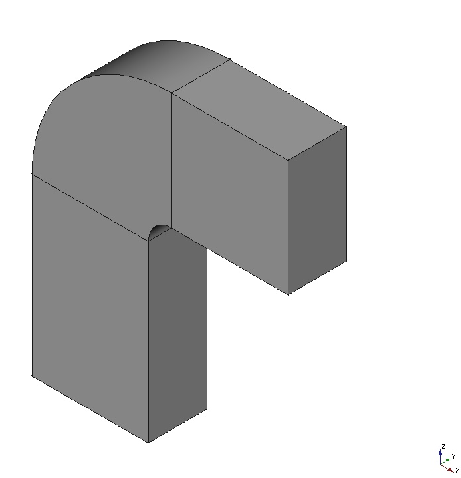
\includegraphics[width=100mm,viewport=0 30 800 270,clip]{geom}
%\caption{Geometry of the step flow problem}\label{fg:struct2b}
%\end{figure}
%


\subsection*{Solution procedure}

The definitions for the relevant equation are not loaded into ElmerGUI by default. Hence, 
one needs to load these before starting the simulations.
\ttbegin
File 
  Definitions
    Append -> k-epsilon.xml
\ttend
The additional definitions should reside in the directory \texttt{edf-extra} within the distribution.\\

Optionally, one may copy the desired \texttt{xml} files to the \texttt{edf}-directory from the 
directory \texttt{edf-extra} which will enable automatic loading of the 
definitions every time ElmerGUI is started. By inspecting the definitions in 
the \texttt{Elmer Definitions File editor} one
may verify that the new definitions were really appended.\newline

The mesh is given in ElmerGrid format in file \texttt{steplong.grd}, load this file.
\ttbegin
File 
  Open -> steplong.grd
\ttend
You should obtain your mesh and may check that it consists of 14584 nodes and of 
14175 bilinear elements.
\ttbegin
Model 
  Summary...
\ttend

After we have the mesh we start to go through the Model menu from the top to bottom. 
In the Setup we choose things related to the whole simulation.
The steady-state simulation is carried out in 2-dimensional Cartesian
coordinates, which are also the defaults.  
The coupled system converges unfortunately quite slowly and hence we need to increase the number of maximum iterations. 
\ttbegin
Model
  Setup 
    Simulation Type = Steady state
    Coordinate system = Cartesian
    Steady state max. iter = 100
\ttend

In the equation section we choose the relevant equations and 
parameters related to their solution. 
In this case the Navier-Stokes and $k-\varepsilon$ equations are needed.
We want to solve the Navier-Stokes and $k-\varepsilon$ equations iteratively using only one non-linear iteration
for optimal convergence of the coupled system. Some relaxation is needed in order to achieve convergence 
at all. We also relax a little bit on the steady state convergence tolerance. 
Initially the Navier-Stokes
solver uses the more robust Picard iteration which may be changed to Newton iteration after the iteration 
progresses. However, here we want to suppress the use of Newton linearisation since it seems to
cause problems with the $k-\varepsilon$ equation.
\ttbegin
Model
  Equation
    Name = Flow equations
    Apply to Bodies = Body 1
    Navier-Stokes 
      Active = on
      Edit Solver Setting
        Nonlinear System
          Max. iterations = 1
          Relaxation factor = 0.5
          Newton after tolerance = 0.0
        Steady state
          Convergence tol. = 1.0e-4
    K-Epsilon 
      Active = on
      Edit Solver Setting
        Nonlinear System
          Max. iterations = 1
          Relaxation factor = 0.5
        Steady state
          Convergence tol. = 1.0e-4
    Add 
    OK
\ttend        

The Material section includes all the material parameters.
They are divided into generic parameters which are direct properties of the material
without making any assumptions on the physical model, such as the density. Other properties assume
a physical law, such as viscosity. For the model parameters of the turbulent equations we are 
happy with the defaults. 
\ttbegin
Model
  Material
    Name = Ideal
    General 
      Density = 1.0
    Navier-Stokes 
      Viscosity = 1.0e-4
      Viscosity Model = K-Epsilon
    Apply to Bodies = Body 1 
    Add
    OK
\ttend

The current case does not have any body forces. To help in the convergence we make 
a rude initial guess.
\ttbegin
Model
  Initial Condition 
    Name = Initial Guess
    Navier-Stokes
      Velocity 1 = 0.0
      Velocity 2 = 0.0
    K-Epsilon
      Kinetic Energy = 0.00457
      Kinetic Dissipation = 1.0e-4
    Apply to Bodies = Body 1 
    Add
    OK
\ttend

When defining Boundary conditions it is possible to assign to the boundaries immediately, or to use mouse
selection to assign them later. In this case we use the latter approach since we do not necessarily know 
the numbering of boundaries by heart.
There is a special boundary condition that takes care of the 
Boundary conditions for the no-slip walls for both the Navier-Stokes and
$k-\varepsilon$ equation. Additionally there are inlet and outlet conditions. 
For the inlet click \texttt{Enter} to open an edit box for the \texttt{Velocity 1} when typing in the expression.
which will be evaluated at run-time so that $v_x=6(y-1)(2-y)$. 
\ttbegin
Model
  BoundaryCondition
    Add 
    Name = Inlet
    Navier-Stokes 
      Velocity 1 = Variable Coordinate 2; Real MATC "6*(tx-1)*(2-tx)"
      Velocity 2 = 0.0
    K-Epsilon
      Kinetic Energy = 0.00457
      Kinetic Dissipation = 1.0e-4
    Add
    New

    Name = Outlet
    Navier-Stokes 
      Velocity 2 = 0.0
    Add 
    New
 
    Name = Walls
    Navier-Stokes 
      Noslip Wall BC = on
    Add
\ttend   

The conditions may also be assigned to boundaries in the Boundary condition menu, or 
by clicking with the mouse. Here we use the latter approach as that spares us of the 
need to know the indexes of each boundary.
\ttbegin
Model
  Set boundary properties
    Choose inlet -> set boundary condition Inlet
    Choose outlet -> set boundary condition Outlet
    Choose walls -> set boundary condition Walls
\ttend

For the execution 
ElmerSolver needs the mesh files and the command file. We have now basically defined
all the information for ElmerGUI to write the command file. After writing it we may also visually 
inspect the command file.
\ttbegin
Sif 
  Generate
  Edit -> look how your command file came out  
\ttend

Before we can execute the solver we should save the files in a directory. The project includes
all the files needed to restart the case. Create a suitable directory for the case if needed. 
\ttbegin
File 
  Save Project
\ttend

After we have successfully saved the files we may start the solver
\ttbegin
Run
  Start solver
\ttend
A convergence view automatically pops up showing relative changes of each iteration.
The convergence if far from monotonic but computation should terminate 
when sufficient convergence is reached after 30 iterations.


\subsection*{Results}

When there are some results to view we may start Paraview for the postprocessing.
\ttbegin
Run
  Paraview
\ttend

The results may be viewed using the postprocessor as shown in 
Figures~\ref{fg:step_ns} and~\ref{fg:step_ke}.
One may also register specific values,
for example the pressure difference is 0.302~Pa, the minimum horizontal and vertical velocities
are -0.213~m/s and -0.0834~m/s, respectively.
One special result of interest 
is the point, on the x-axis, at which the direction of the flow changes. 
In this case its position is about 5.1~m after the step. 

\begin{figure}[h]
\centering
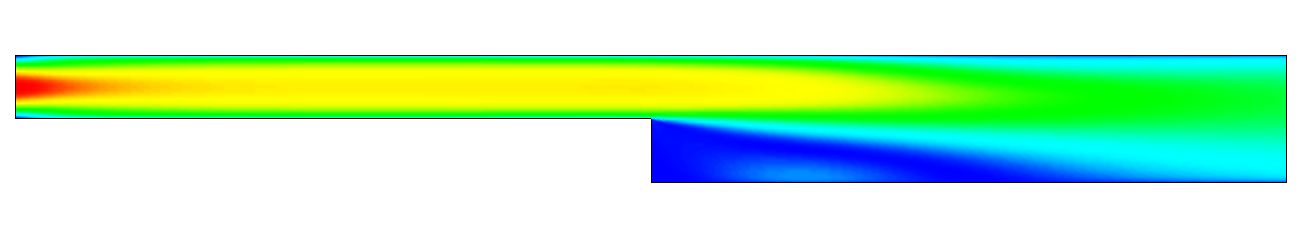
\includegraphics[width=15cm]{step_ke_velo}
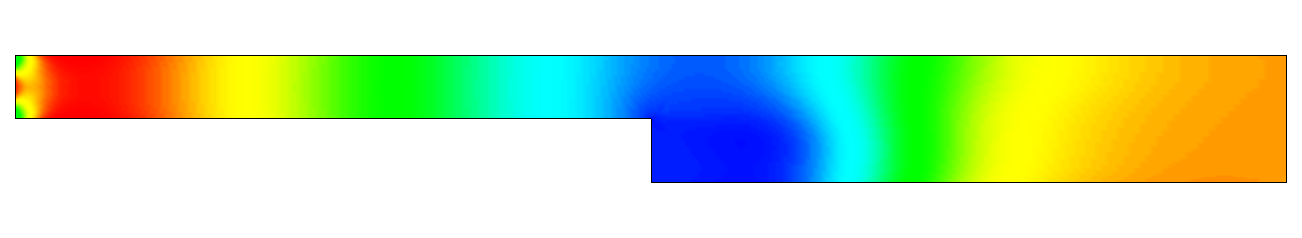
\includegraphics[width=15cm]{step_ke_pres}
\caption{Variables of the Navier-Stokes solver: absolute velocity on top and 
pressure on bottom}\label{fg:step_ns}
\end{figure} 

\begin{figure}[h]
\centering
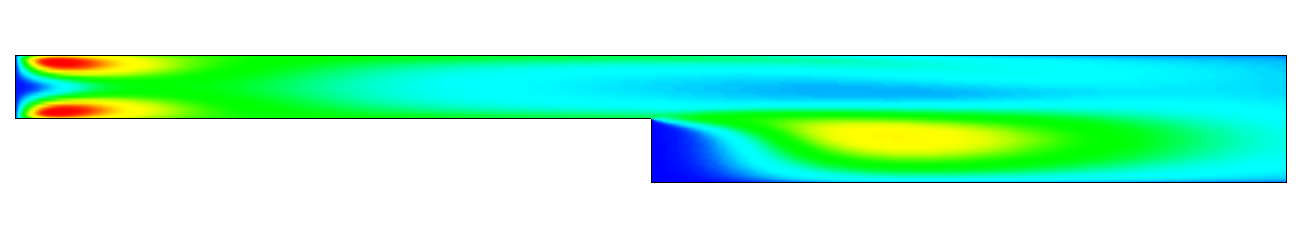
\includegraphics[width=15cm]{step_ke_kin}
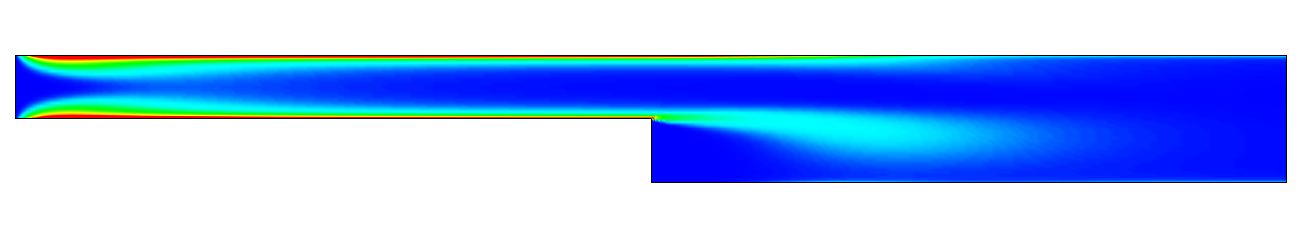
\includegraphics[width=15cm]{step_ke_diss}
\caption{Variables of the $k-\varepsilon$ solver: kinetic energy on top and its dissipation on bottom}
\label{fg:step_ke}
\end{figure} 


\hfill
